\documentclass[leqno,presentation]{beamer}

\usepackage[orientation=landscape, size=a0, scale=1.3]{beamerposter}
\usepackage{pgf}
\usepackage{tikz}
\usepackage{calc}
\usepackage{times}
\usepackage{type1cm}
\usepackage[latin1]{inputenc}

\usepackage{amsmath,amssymb, latexsym}
\usepackage[english]{babel}

\usetheme{Darmstadt}

\title{
\veryHuge
Point-Pushing Homeomorphisms on a Genus-$g$ Surface}
  \author{
  \LARGE
  Victor Yang,
  Xiaolong Han,
  Yohan Kang,
  Joe Nance,
  Spencer Dowdall (Faculty Mentor)}
  
\institute{
\raisebox{-2ex}{
\includegraphics[width=5in]{uiuc_logo.pdf}}
\hspace{4em}
\raisebox{-2ex}{
\includegraphics[width=1in]{igl-logo-small.png}}
\hspace{1em} 
{\Large\textcolor{red!50!orange}{ Illinois Geometry Lab}}
}

\date{\large IGL Open House, December 11, 2014}

\begin{document}

\begin{frame}

\begin{block}{}
\titlepage
\end{block}

\begin{columns}[t]

\begin{column}[t]{.25\linewidth}

\begin{block}{Point-Pushing Homeomorphisms}
\vspace{1ex}
\begin{itemize}
	
\item {[Definition]}: Each closed curve $\gamma$ with a base point $pt$ on a surface $S$ determines a natural homeomorphism $\mathcal{P}(\gamma)$ of the surface $S\setminus\{pt\}$ via \textbf{point-pushing}:
\vspace{1ex}
\begin{figure}[h]
	\begin{center}
		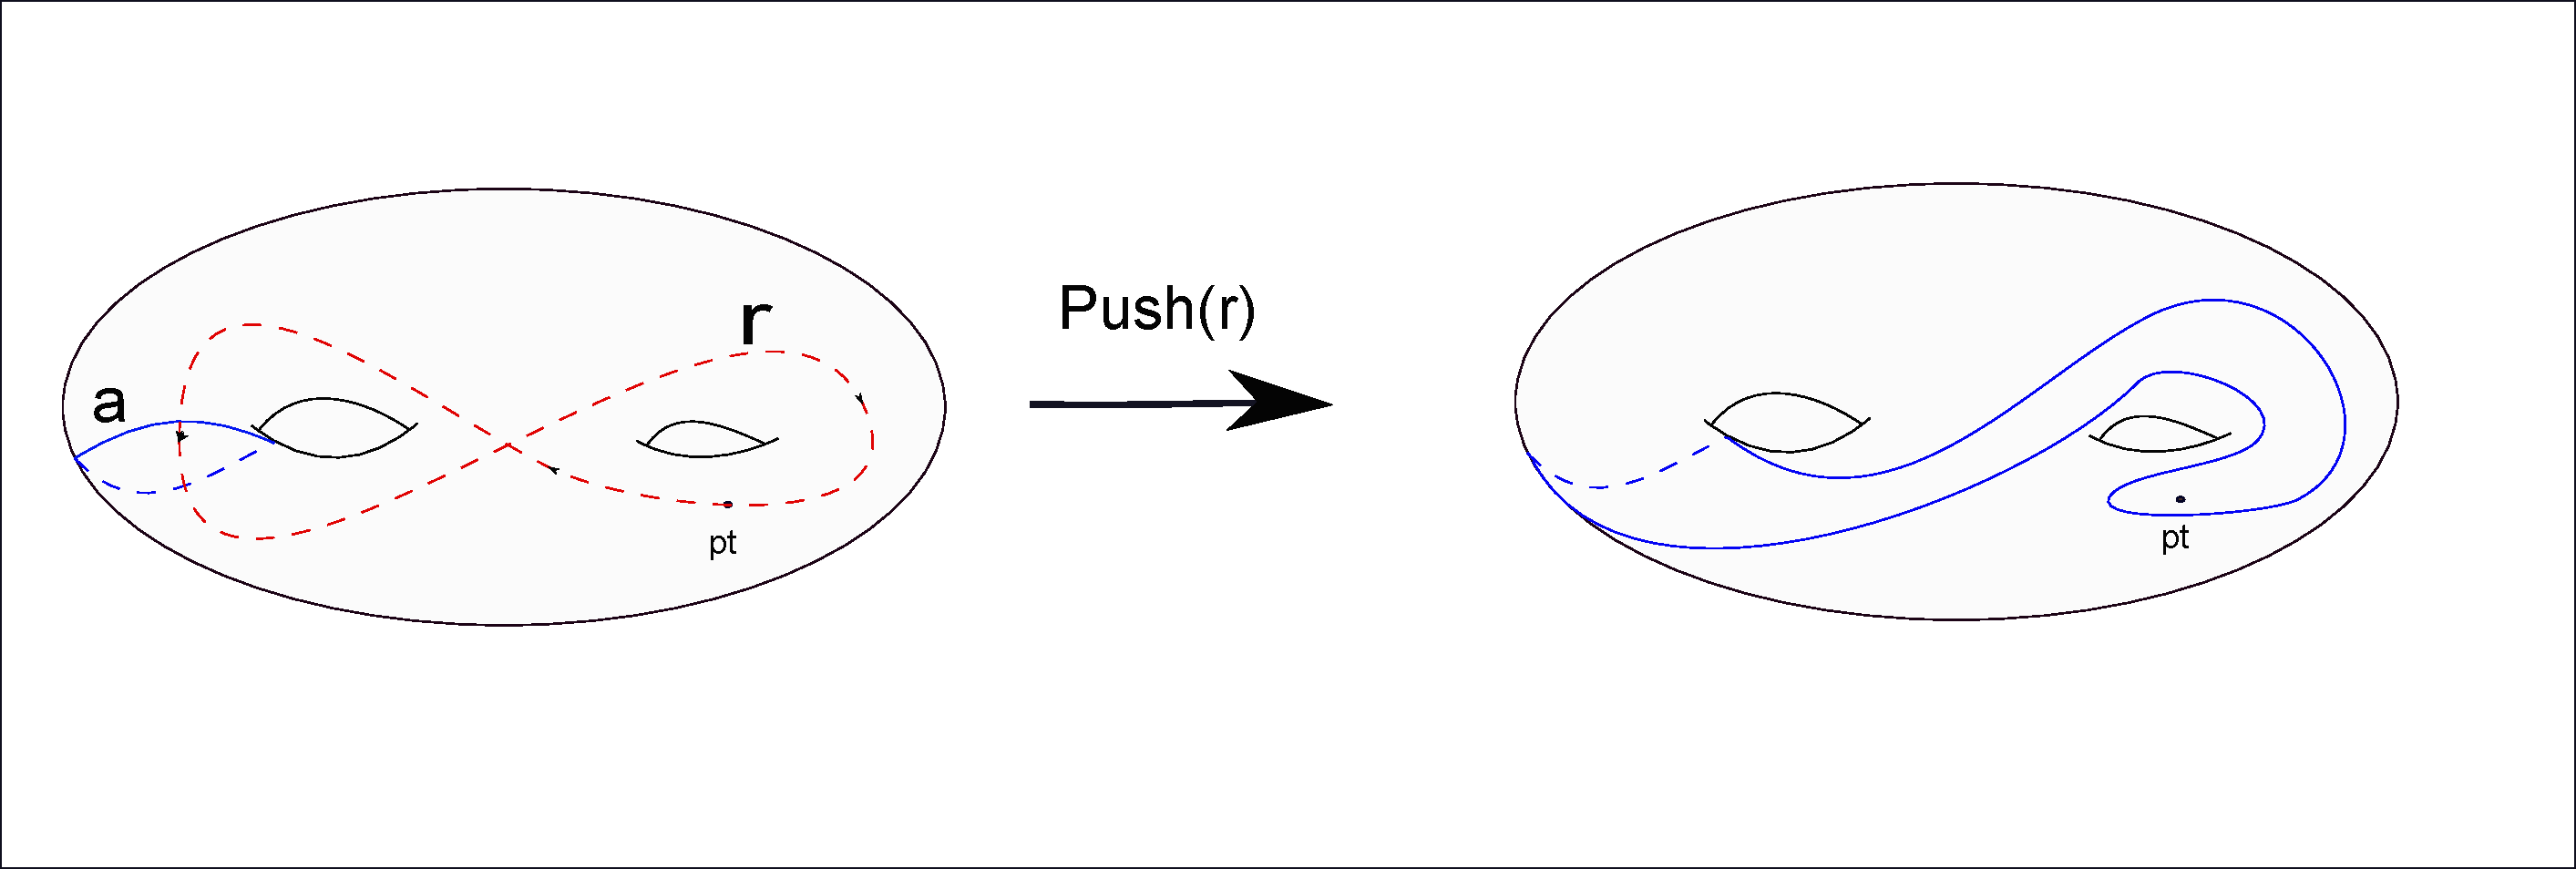
\includegraphics[width=11in]{Ex_Point-Pushing_Homeomorphism.pdf}
		\caption{{\bf Point-push} around $\gamma$ by dragging basepoint $pt$ once around $\gamma$.}
	\end{center}
\end{figure}

\item {[Theorem]}: Every point-pushing homeomorphism on a genus-$g$ surface with a base point $p\in S$ can be written as a composition of \textit{generating} point-pushing homeomorphisms and their inverses.
\vspace{1ex}

\end{itemize}
\end{block}

\begin{block}{Self-Intersection Numbers}
\vspace{1ex}
\begin{itemize}
\item {[Definition]} Let $\gamma$ be a closed curve on a surface $S$ and $[\gamma]$ be the homotopy class of $\gamma$. The self-intersection number of $\gamma$ is the minimum of the set of all self-intersection numbers of curves in $[\gamma]$. i.e., the minimum of the set of all self-intersection numbers of the curves that are homotopic to $\gamma$. (For example, the self-intersection number of $\gamma$ in the figure above will be at most $1$.)
\end{itemize}
\end{block}

\end{column}

\begin{column}{.45\linewidth}

\begin{block}{Brief Description of Our Project}
\vspace{1ex}
\underline{Goal}

The goal of this project is to study point-pushing homeomorphisms on the genus-$g$ surface, and to relate their topological entropy (mesured by Dilatation) to their combinatorial complexity (mesured by Self-Intersection Number).
 
\underline{Procedure (Algorithm for our computer program)}

1. Randomly pick a closed curve $\gamma$ with a base point $pt$ on a Genus-$g$ surface. (We choosed $g$ to be $2$.)

~~~~~And let $\mathcal{P}(\gamma)$ be the associated point-pushing homeomorphism around $\gamma$.

2. Express $\mathcal{P}(\gamma)$ as a composition of generating dehn-twists in order to calculate its topological entropy.

3. Calculate the Self-Intersection Number of $\gamma$ and the Dilatation of $\mathcal{P}(\gamma)$.

4. Repeat this process, enough times, so that we can get enough data.

5. Analyze the distribution of the Self-Intersection Numbers of randomly selected closed curves.

6. Analyze the distribution of the Dilataion of randomly selected point-pushing homeomorphisms.

8. Analyze the correlation between the Self-Intersection Numbers and Dilatation.

\end{block}
%%%%%%%%%%%%%%%%%%%%%%%%%%%%%%%%%%%%%%
% end center block 1
%%%%%%%%%%%%%%%%%%%%%%%%%%%%%%%%%%%%%%

%%%%%%%%%%%%%%%%%%%%%%%%%%%%%%%%%%%%%%
% center block 2
%%%%%%%%%%%%%%%%%%%%%%%%%%%%%%%%%%%%%%
\begin{block}{Distribution of Dilatations and Self-Intersection Numbers in the Genus-$2$ surface}
\vspace{1ex}
\begin{figure}
		\includegraphics[width=10in]{G2L12.jpg}
		\caption{Distribution of Topological Entropies of randomly selected point-pushing homeomorphism on genus-$2$ surface.}
\end{figure}
\end{block}
%%%%%%%%%%%%%%%%%%%%%%%%%%%%%%%%%%%%%%
% end center block 2
%%%%%%%%%%%%%%%%%%%%%%%%%%%%%%%%%%%%%%

%%%%%%%%%%%%%%%%%%%%%%%%%%%%%%%%%%%%%%
% center block 3
%%%%%%%%%%%%%%%%%%%%%%%%%%%%%%%%%%%%%%
\begin{block}{Correlation between Dilatations and Self-Intersection Numbers in the Genus-$2$ surface, and Analysis }
\vspace{1ex}
\begin{figure}
	\includegraphics[width=10in]{G2L12_Scatter_Plot.jpg}
	\caption{Scatter plot of Self-Intersection Number vs Topological Entropies of randomly selected point-pushing homeomorphism on genus-$2$ surface.}
\end{figure}
\end{block}
%%%%%%%%%%%%%%%%%%%%%%%%%%%%%%%%%%%%%%
% end center block 3
%%%%%%%%%%%%%%%%%%%%%%%%%%%%%%%%%%%%%%

\end{column}

%%%%%%%%%%%%%%%%%%%%%%%%%%%%%%%%%%%%%%%%%%%%%%%%%%%%%%%%%%%%%%%%%%%%%%%%%
% end middle column, wide
%%%%%%%%%%%%%%%%%%%%%%%%%%%%%%%%%%%%%%%%%%%%%%%%%%%%%%%%%%%%%%%%%%%%%%%%%


%%%%%%%%%%%%%%%%%%%%%%%%%%%%%%%%%%%%%%%%%%%%%%%%%%%%%%%%%%%%%%%%%%%%%%%%%
% right column, narrow 
%%%%%%%%%%%%%%%%%%%%%%%%%%%%%%%%%%%%%%%%%%%%%%%%%%%%%%%%%%%%%%%%%%%%%%%%%

\begin{column}{.25\linewidth}

%%%%%%%%%%%%%%%%%%%%%%%%%%%%%%%%%%%%%%
% right block 1
%%%%%%%%%%%%%%%%%%%%%%%%%%%%%%%%%%%%%%
\begin{block}{Dehn-Twists}
	\vspace{1ex}
	\begin{itemize}
		\item {[Definition]}: A dehn-twsit about a closed curve $\gamma$ on a surface $S$ is a self-homeomorphism on $S$ that can be obtained by twsiting $2\pi$ about the given curve $\gamma$.

		\item {[Theorem]}: Every homeomorphism on a genus-$g$ surface can be written as a composition of \textit{generating} dehn-twists (about the following generating curves in the picture below) and their inverses.
		\vspace{1ex}
		\begin{figure}[h]
			\begin{center}
				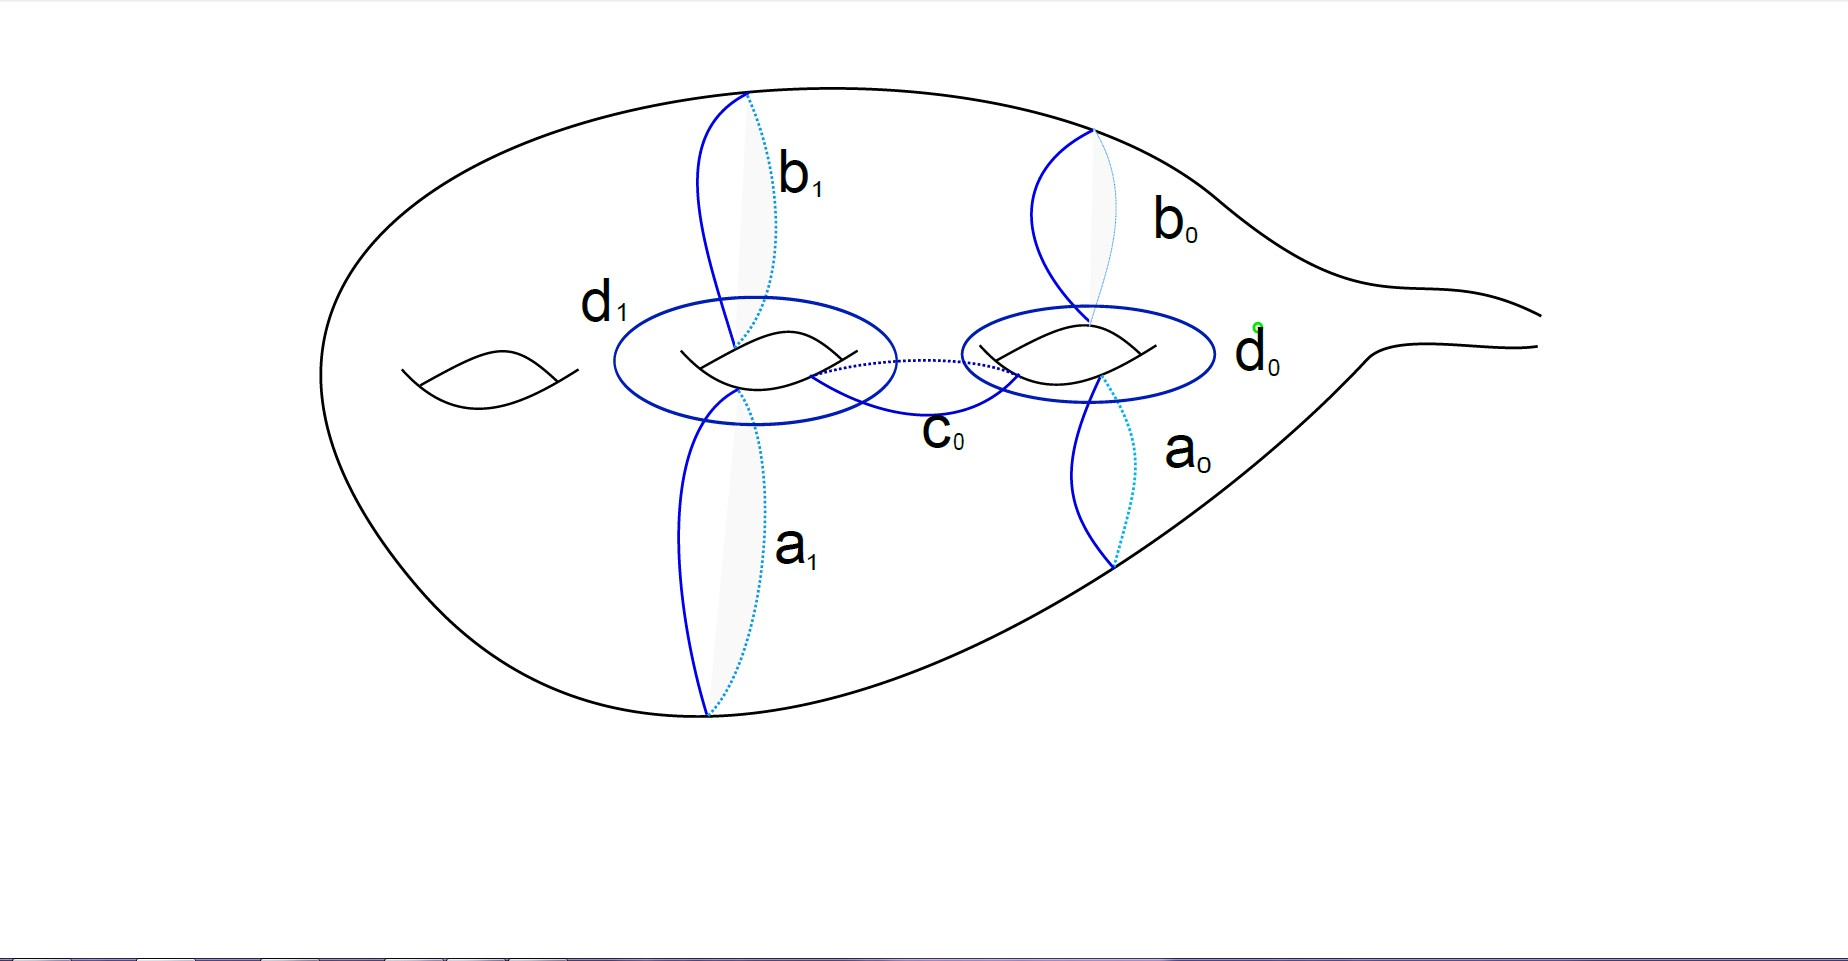
\includegraphics[width=11in]{Ex_Dehn-Twist_Generating_Curves.jpg}
				\caption{Example of Generating Cuves on a genus-$g$ surface.}
			\end{center}
		\end{figure}
		\item {[Consequence]} Every point-pushing homeomorphism on a surface can be written as a product of some "generating" point-pushing homeomorphisms, which then, can be written as a product of some "generating" Dehn-Twists.
	\end{itemize}
\end{block}
%%%%%%%%%%%%%%%%%%%%%%%%%%%%%%%%%%%%%%
% end right block 1
%%%%%%%%%%%%%%%%%%%%%%%%%%%%%%%%%%%%%%

%%%%%%%%%%%%%%%%%%%%%%%%%%%%%%%%%%%%%%
% right block 2
%%%%%%%%%%%%%%%%%%%%%%%%%%%%%%%%%%%%%%
\begin{block}{Topological Entropy}
\vspace{1ex}
\begin{itemize}
\item {[Definition]} Topological entropy is a nonnegative number which measures the complexity of a topological dynamical system. In this project, the topological dynamical system will be a surface with a point-pushing homeomorphism on that surface. Moreover, we measured the topological entropy of a point-pushing homeomorphism on a surface with the dilatation number of the given homeomorphism, so that the topological entropy of the given homeomorphism would be the logorithm of the dilatation.
\end{itemize}
\end{block}
%%%%%%%%%%%%%%%%%%%%%%%%%%%%%%%%%%%%%%
% end right block 2
%%%%%%%%%%%%%%%%%%%%%%%%%%%%%%%%%%%%%%

%%%%%%%%%%%%%%%%%%%%%%%%%%%%%%%%%%%%%%
% right block 3
%%%%%%%%%%%%%%%%%%%%%%%%%%%%%%%%%%%%%%

%%%%%%%%%%%%%%%%%%%%%%%%%%%%%%%%%%%%%%
% end right block 3
%%%%%%%%%%%%%%%%%%%%%%%%%%%%%%%%%%%%%%

\end{column}
%%%%%%%%%%%%%%%%%%%%%%%%%%%%%%%%%%%%%%%%%%%%%%%%%%%%%%%%%%%%%%%%%%%%%%%%%
% end right column
%%%%%%%%%%%%%%%%%%%%%%%%%%%%%%%%%%%%%%%%%%%%%%%%%%%%%%%%%%%%%%%%%%%%%%%%%

\end{columns}
%%%%%%%%%%%%%%%
%Funding Acknowledgements: Make sure you get this right before sending to printers
%%%%%%%%%%%%%%%
  \begin{block}{}
   \begin{center}
   These posters are made with the support of University of Illinois at Urbana-Champaign Public Engagement Office
  \end{center}
  \end{block}



\end{frame}
\end{document}